\section{Elektriska grundbegrepp}

\harec{a}{1.1}

Elektrisk laddning, spänning och ström hänger samman med hur materian är
uppbyggd.
Den förmåga ett material har att leda laddningar, d.v.s. ström, kallas
konduktivitet.

\subsection{Grundämnen}
\textbf{FÖRDJUPNING}
\index{grundämnen}

Det finns många former av materia.
Ofta är en form av materia sammansatt av andra former med enklare uppbyggnad.

Sammansatt materia kan sönderdelas på kemisk väg, men däremot inte de enklaste
formerna.
All materia är uppbyggd av atomer.
De enklaste materieformerna, som kallas \emph{grundämnen}, innehåller endast
ett slags atomer.
Över 100~grundämnen är kända.

Vart och ett av grundämnena har sin speciella atomuppbyggnad och därmed en
materialstruktur, som skiljer sig från varje annat grundämne.

Tre fjärdedelar av alla grundämnen är metaller (elektriska ledare) medan de
flesta övriga är icke-metaller (isolatorer).
Det finns även en liten mellangrupp som kallas för halvledare.

\subsection{Atomernas uppbyggnad}
\textbf{FÖRDJUPNING}

Länge ansågs atomerna vara de minsta beståndsdelarna i materian.
Men omkring sekelskiftet upptäcktes att atomerna i sin tur består av ännu mindre
beståndsdelar, s.k. elementarpartiklar såsom protoner, neutroner, elektroner
m.fl.
Det gemensamma namnet för alla dessa partiklar är \emph{nukleoner}.

En atom består dels av en kärna, som är sammansatt av protoner och neutroner,
dels av elektroner, som kretsar omkring kärnan.

\begin{quote}
\emph{Protonerna är positivt (+) laddade.}

\emph{Neutronerna är neutrala, ej laddade.}

\emph{Elektronerna är negativt (-) laddade}
\end{quote}

\begin{wrapfigure}{L}{0.5\textwidth}
  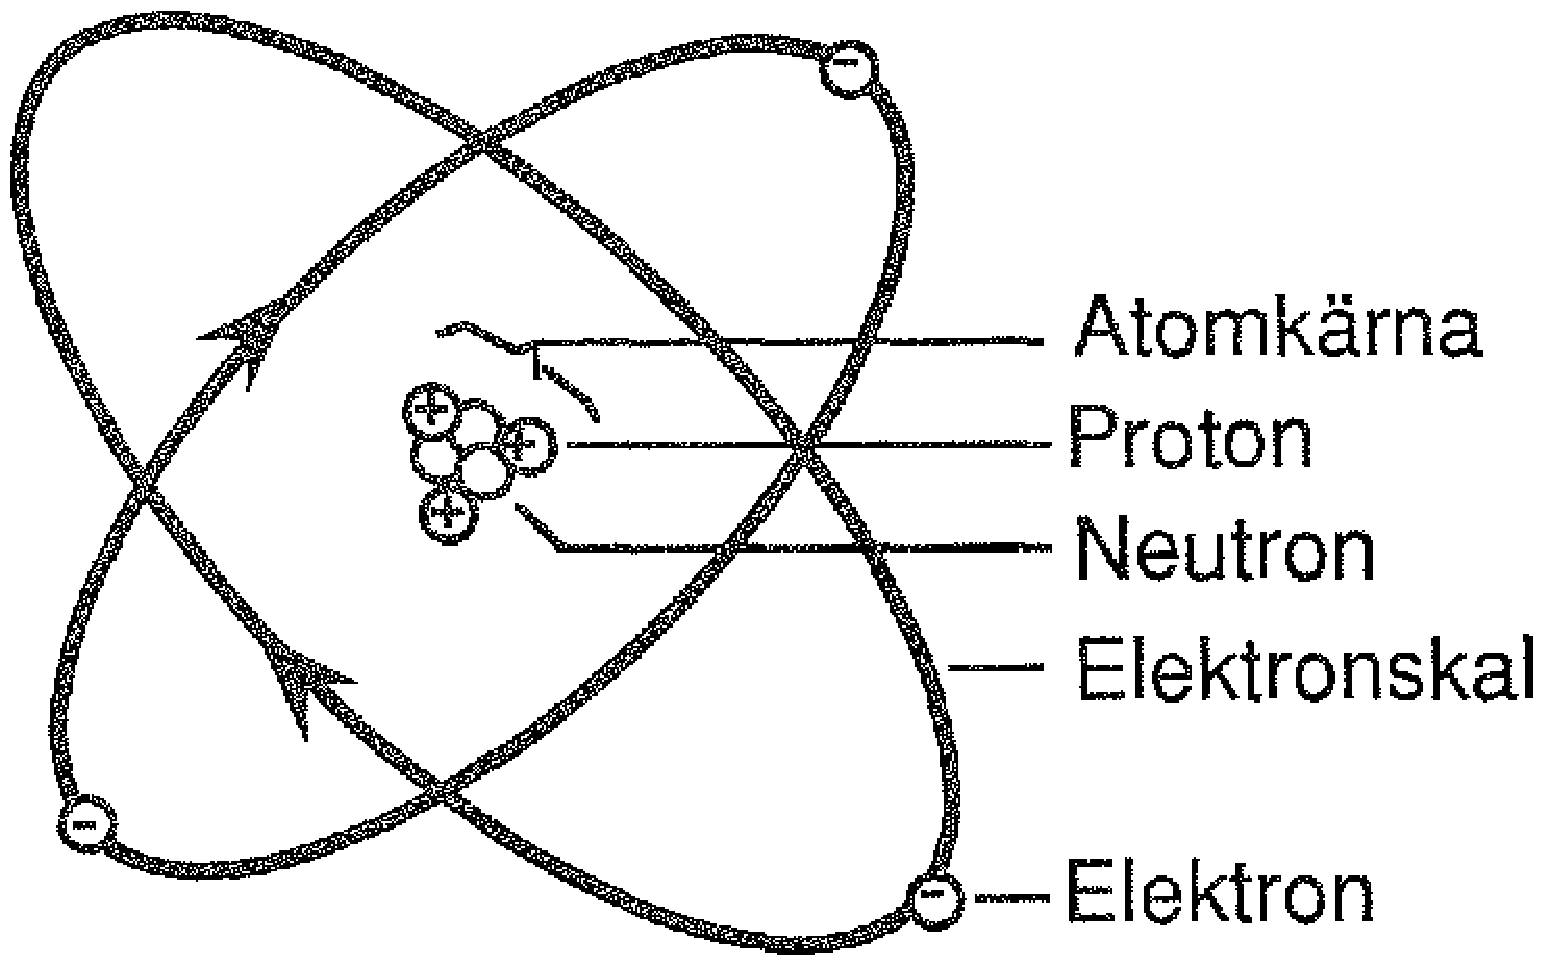
\includegraphics[width=0.5\textwidth]{images/cropped_pdfs/bild_2_1-01.pdf}
  \caption{Atomernas uppbyggnad}
  \label{fig:BildII1-1}
  \vspace{-20pt}
\end{wrapfigure}

Elektronerna kretsar i banor omkring atomkärnorna, liksom
planeterna kretsar i banor omkring sina solar, vilket illustreras i bild
\ref{fig:BildII1-1}.

Banor med samma avstånd till atomkärnan är på samma energinivå och sägs bilda
ett elektronskal.

Det kan finnas flera elektronskal.
Ju fler elektroner som finns i ett elektronskal, desto starkare är elektronerna
i skalet bundna till atomen.
Det yttersta skalet kan emellertid aldrig innehålla fler än 8~elektroner.

Elektronerna i det yttersta skalet kallas för \emph{valenselektroner}, vilka
används även av angränsande atomer vid den kemiska bindningen till
atomstrukturer, molekyler och ämnen.
För bindningen behövs ett visst antal valenselektroner.

De valenselektroner som ej behövs för bindningen kan röra sig fritt genom
materia/strukturen.
De kallas fria elektroner och är vad vi kallar elektrisk ström.

Valenselektronerna är alltså inte bara av betydelse för materialets kemiska
struktur utan också för dess elektriska egenskaper.

Atomernas massa och volym är ytterst liten.
Tag som exempel en kub av koppar med volymen \(1\ cm^3\) och vikten
\(8,9\ gram\).
Den består av ca \(8,5 \cdot 10^{25}\) kopparatomer, d.v.s.
\(85\, 000\, 000\, 000\, 000\, 000\, 000\, 000\, 000\) stycken.

Varje elementarpartikel har en massa och en atoms totala massa är summan av
elementarpartiklarnas massor.
Den enklaste atomen är väteatomen med en proton och en elektron.
Väteatomens totala massa har kunnat beräknas till \(1,66 \cdot 10^{-24}\) gram.

Nästan hela massan i atomen är samlad till kärnans protoner och neutroner.
Var och en av dem har en massa som är ungefär 2000 gånger större än massan i en
elektron.
\(1\ cm^3\) av koppar innehåller t.ex. \(10^{23}\) stycken fria elektroner.

\subsection{Elektrisk laddning och kraftverkan}
\textbf{FÖRDJUPNING}
\index{elektrisk laddning}

Enligt sägnen upptäckte Thales från Milteus redan för 2500~år sedan, att en bit
bärnsten drog till sig små grässtrån, sedan stenen gnidits mot en bit ylle.
Det grekiska ordet för bärnsten är ELEKTRON och de krafter som uppstod kom att
kallas ''elektriska''.
Av den elektriska spänningen mellan kroppar med olika laddning, verkar krafter
mellan dem och deras omgivning.
Krafterna kallas för elektriska fält och är det som gör att elektriskt laddade
kroppar kan komma i rörelse.

Ett exempel får man varje gång man kammar sig med en kam av isolerande material.
Då kommer håret att dras mot kammen därför att håret och kammen har
fått olika slags elektriska laddningar.
Samtidigt har hårstråna sinsemellan samma slags laddning och stöter bort
varandra -- håret ''reser sig''.

Lika laddningar stöter bort varandra.

Olika laddningar drar varandra till sig.

\subsection{Konduktivitet -- Ledare, halvledare och isolator}
\textbf{HAREC a.\ref{HAREC.a.1.1.1}\label{myHAREC.a.1.1.1}}
\index{konduktivitet}

En elektrisk ström sägs flyta, när de fria laddningsbärarna i ett material -- en
strömledare -- fås att röra sig samtidigt i samma riktning.
Hur många som rör sig beror på strömledarens egenskaper och spänningen mellan
ledarens ändar.

Alla material har någon grad av elektrisk ledningsförmåga som beror på
materialets atomstruktur, dimensioner och temperatur.
Vissa material (t.ex. metaller, kol, halvledare) leder elektrisk ström bättre
än andra (t.ex. glas, gummi, plast).
Mängden av fria laddningsbärare i materialet begränsar hur stor strömmen kan
bli.

\subsubsection{Ledare}
\index{ledare}
\index{konduktivitet!ledare}

Metaller har god elektrisk ledningsförmåga och kallas ledare.
Bäst ledande är de metaller, vars atomer har det minsta antalet
valenselektroner i det yttersta elektronskalet.
Koppar-, silver- och guldatomerna har en enda valenselektron och därmed mycket
god ledningsförmåga.
Järn, zink och magnesium har två valenselektroner och därmed något sämre
ledningsförmåga.
Ännu sämre ledare är de s.k. halvledarna med 3 till 5 valenselektroner.

\subsubsection{Isolatorer}
\index{isolator}
\index{konduktivitet!isolator}

Glas, plast, porslin och vissa mineraler har mycket dålig ledningsförmåga och
kallas isolatorer.
Isolatorerna är dåliga ledare på grund av att de har många valenselektroner i
sitt yttersta skal.
Maximalt ryms 8 valenselektroner.

I icke ledande material är elektronerna mycket hårt bundna till sitt valensskal
och därför svåra att flytta.
I fasta material är också positiva laddningar svåra att flytta, eftersom de är
bundna i atomkärnorna.
Atomerna är i sin tur bundna i en struktur som kännetecknar vart och ett
material.

\subsubsection{Halvledare}
\index{halvledare}
\index{konduktivitet!halvledare}

En ren kristall av mineralen germanium [Ge] eller av kisel [Si] leder
inte elektrisk ström.
Båda dessa mineral är därför isolatorer.
Om några atomer av ett främmande material blandas in i deras kristaller, så
blir de i någon mån elektriskt ledande -- de blir halvledare.
Inblandningen är 1 eller 2 främmande atomer per 100 miljoner germanium- eller
kiselatomer.
Liknande resultat fås med andra material.
Beroende på materialen och i vilka proportioner de blandas fås olika egenskaper.

\subsubsection{N-ledning}
Man talar om N-ledande material respektive N-ledning- ''elektronledning''.

Germanium, kisel m.fl. halvledare har fyra elektroner med ''fasta platser'' i
valensskalet -- förutsatt att materialet är helt rent.
Då finns det inga fria elektroner för laddningstransport.

För att skapa fria elektroner kan det rena materialet förorenas -- dopas -- med
atomer av t.ex. arsenik [As] eller antimon [Sb].
Båda dessa material är 5-värdiga.
De har 5 elektroner i valensskalet 4 elektroner är fast bundna medan
den 5:e är löst bunden till atomen.
Den 5:e elektronen kan lossgöras från atomen med yttre kraft, t.ex. värme eller
elektrisk spänning och då skapas en fri elektron.
När en spänning läggs på materialet kommer den fria elektronen att vandra mot
den positiva polen.
Materialet är N-ledande.

\subsubsection{P-ledning -- ''hålledning''}
När germanium eller kisel dopas med indium [In] eller gallium [Ga] så blir de
P-ledande.
Indium och gallium är 3-värdiga -- deras valensskal innehåller 3 elektroner.
Men för en fast bindning med germanium eller kisel saknas det en elektron och
det uppstår då ett ''hål'' -- en ''bristelektron''.
Hålet kan fyllas ut av en elektron från en annan atom.
I den atom som elektronen lämnar bildas det i sin tur ett hål o.s.v.
När en spänning läggs på, kommer ''hålet'' att vandra mot den negativa polen.
Materialet är då P-ledande.

\subsection{Elektrisk spänning -- Enheten Volt}
\textbf{HAREC a.\ref{HAREC.a.1.1.2}\label{myHAREC.a.1.1.2b}, a.\ref{HAREC.a.1.1.3}\label{myHAREC.a.1.1.3b}}
\index{elektrisk spänning}
\index{spänning}
\index{Volt (V)}
\index{enheter!Volt (V)}
\index{symbol!\(U\) spänning}
\index{symbol!\(V\) spänning}

\begin{figure*}
\begin{center}
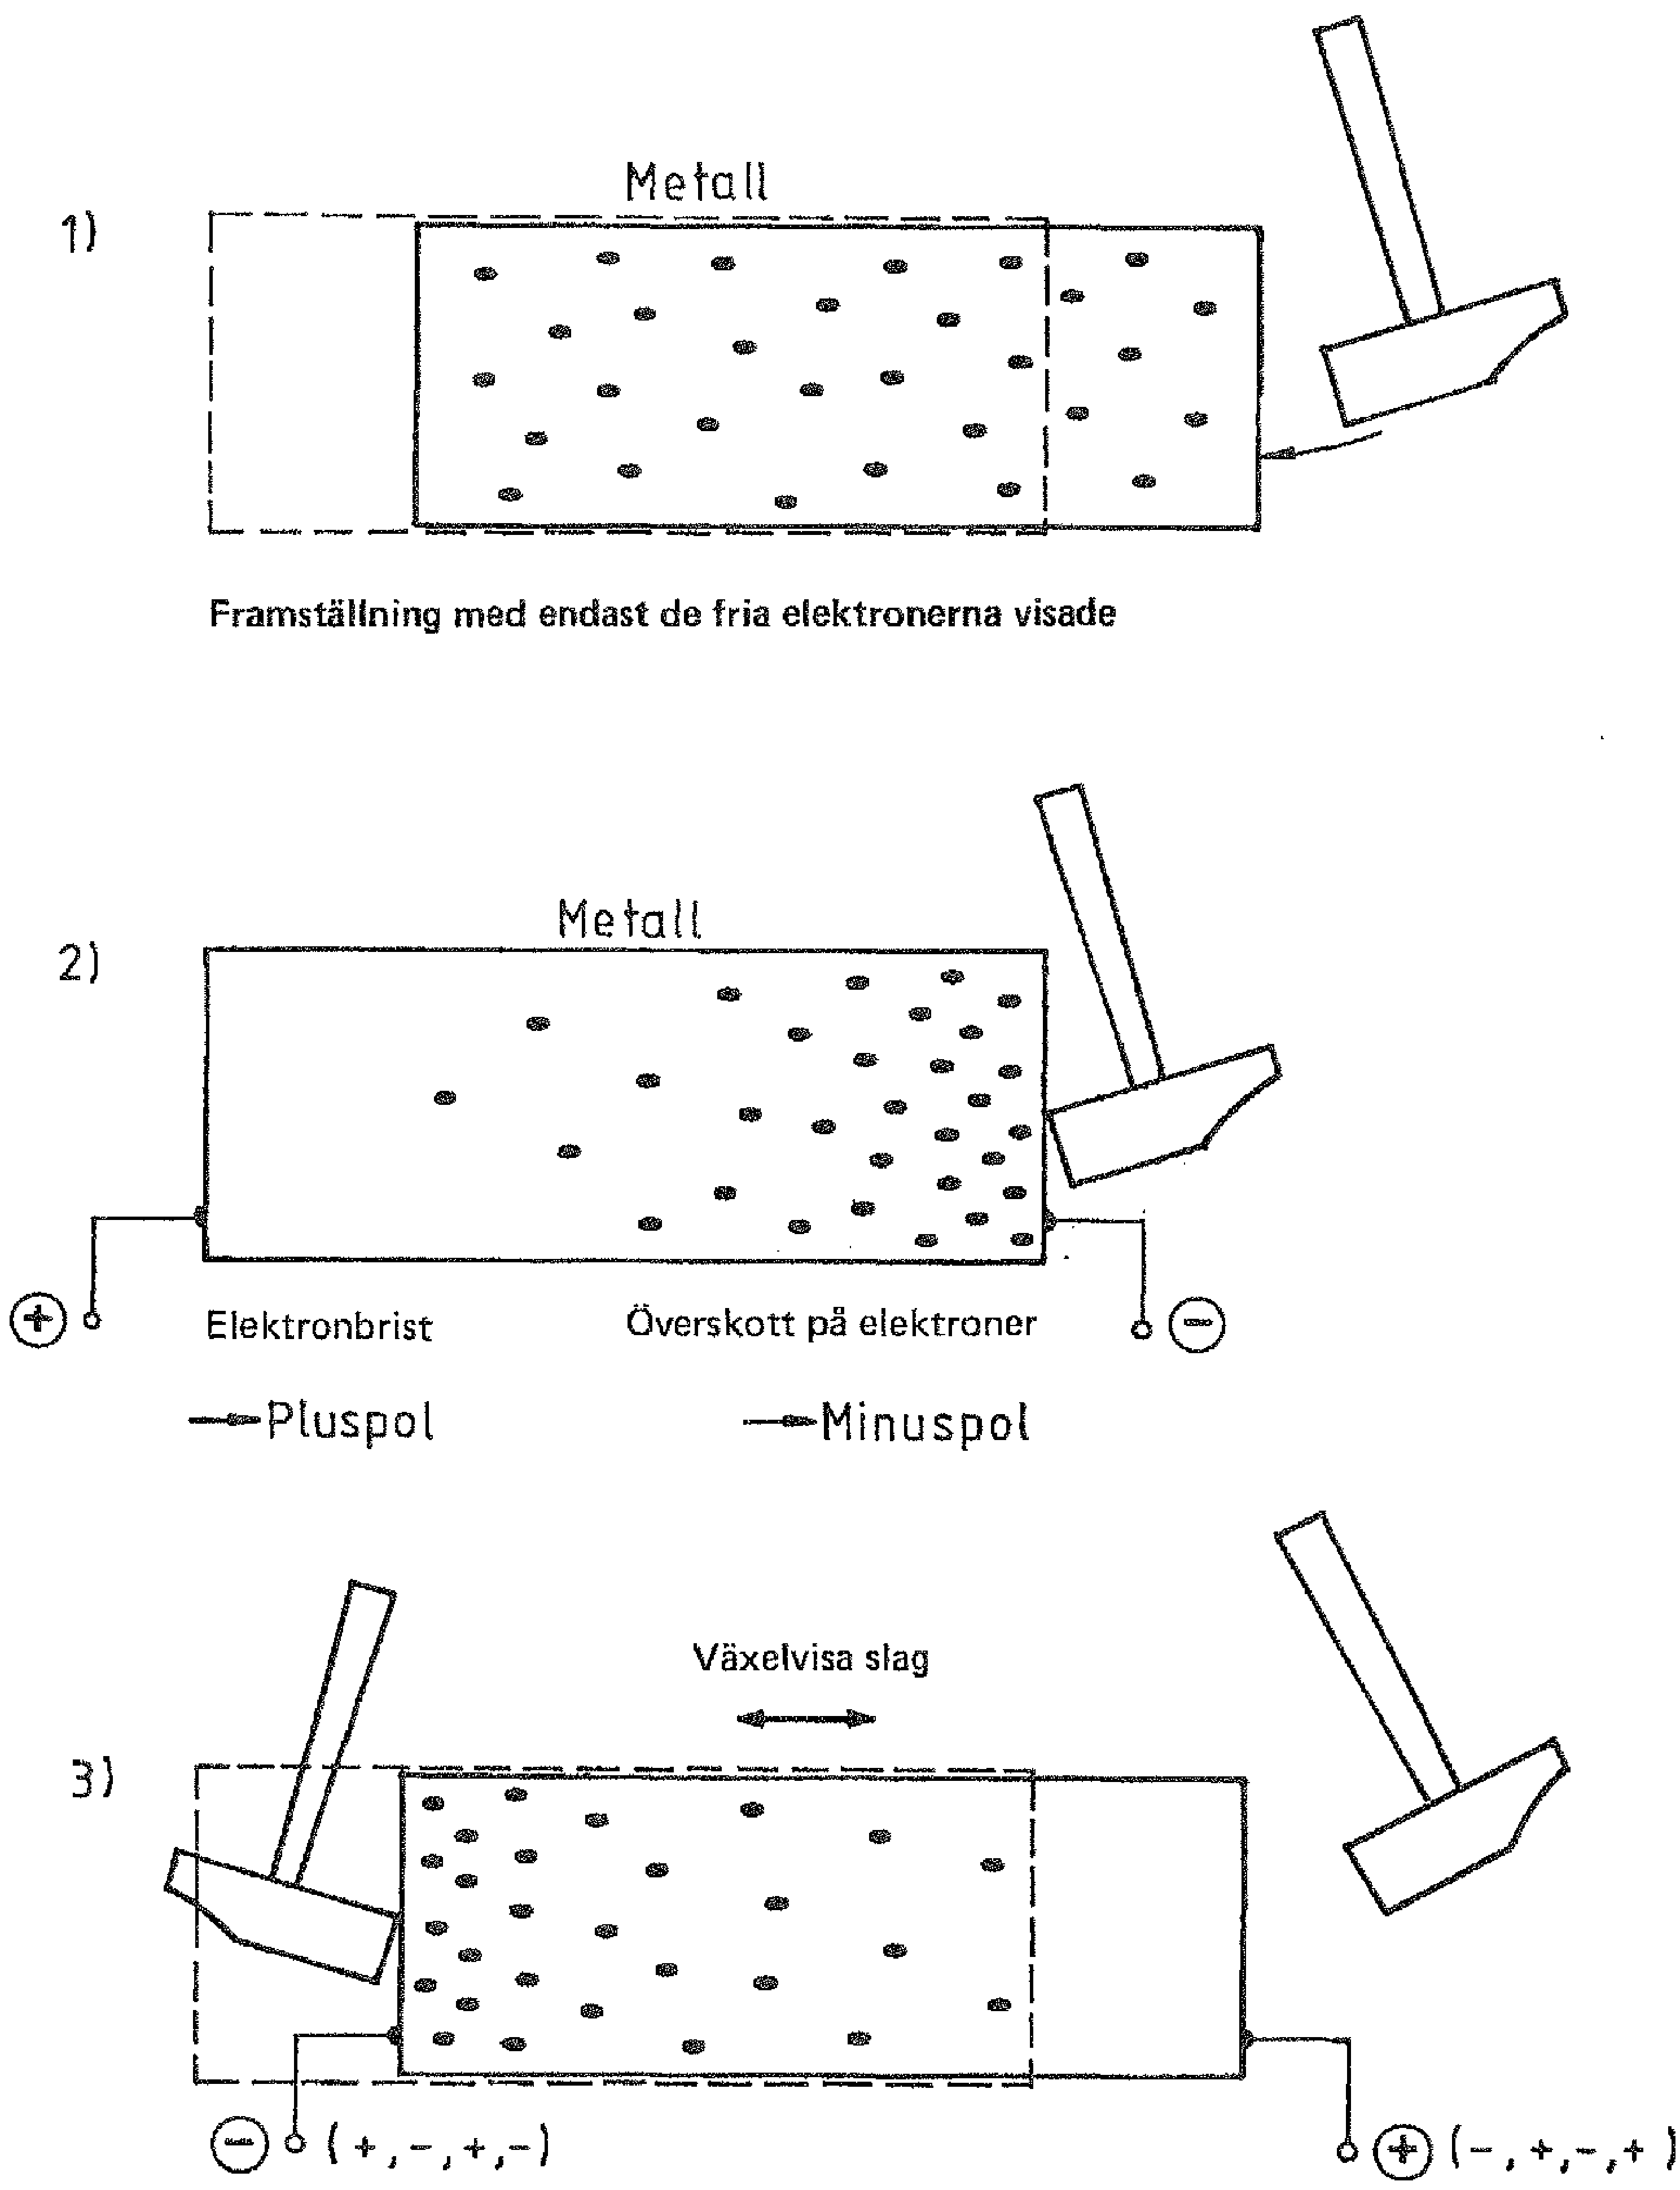
\includegraphics[width=\textwidth]{images/cropped_pdfs/bild_2_1-02.pdf}
\caption{Tankeförsök med kulor i ett rör}
\label{fig:BildII1-2}
\end{center}
\end{figure*}

Bild \ref{fig:BildII1-2} illustrerar ett tankeförsök med ett rör med kulor i,
tänks materialet i röret motsvara atomstrukturen i en strömledare och kulorna
de fria elektronerna.
Tänker man sig ett slag mot en ände av röret så flyttar det sig av den energi
som tillförs.
På grund av obundenheten till röret så följer av masströgheten kulorna inte med
röret, utan hamnar i dess ena ände.

Att kulorna samlas i ena änden av röret tänks motsvara ett elektronöverskott i
ena änden av en ledare och ett motsvarande underskott i den andra änden.

Man kallar änden med elektronöverskott för minuspol och änden med
elektronunderskott för pluspol.
Olika stora elektriska laddningar vid polerna innebär att de sinsemellan har
olika potential.
Potentialskillnaden kallas spänning.

Likspänning innebär ett överskott av elektroner och alltid vid samma
anslutningspol.

Växelspänning innebär ett överskott av elektroner, omväxlande vid den ena
anslutningspolen och den andra.

Måttenheten för spänning är \(Volt\ [V]\).
I formler betecknas spänning med
\begin{itemize}
  \item \(U\) för effektivvärdet
  \item \(u\) för momentanvärdet (ögonblicks-)
  \item \(\hat{u}\) för toppvärdet (amplitud-).
\end{itemize}

Spänningen över ändpunkterna på en strömledare är \(1\ Volt\ [V]\), då
ledaren genomflyts av en likström av \(1\ Ampere\ [A]\) under
effektutvecklingen \(1\ Watt\ [W]\).

\subsection{Symboler}

\begin{wrapfigure}[6]{R}{0.4\textwidth}
  \begin{mdframed}
    \centering
    \begin{circuitikz}
      \draw
      (4,1) to[battery1] (1,1)
      ;
    \end{circuitikz}
    \caption{Schemasymbol för batteri}
    \label{fig:bildII2-batteri}
  \end{mdframed}
\end{wrapfigure}

\textbf{FÖRDJUPNING}

När man ritar scheman för elektriska kretsar, används symboler.
Symbolen i bild \ref{fig:bildII2-batteri} visar ett elektriskt batteri med en
enda cell.

Förtydligande kommentarer och skrivtecknen invid symbolen förekommer.
Ofta refererar dessa till en komponentlista.
Se även kapitel \ref{komponenter}.

\subsection{Elektrisk ström -- Enheten Ampere}
\textbf{HAREC a.\ref{HAREC.a.1.1.2}\label{myHAREC.a.1.1.2a}, a.\ref{HAREC.a.1.1.3}\label{myHAREC.a.1.1.3a}}
\index{elektrisk ström}
\index{ström}
\index{Ampere (A)}
\index{enheter!Ampere (A)}
\index{symbol!\(I\) ström}

När en sluten strömkrets innehåller en spänningskälla, så kan en
laddningsutjämning ske genom kretsen.
Det innebär att fria elektroner förflyttar sig genom kretsen i riktning från
spänningskällans minuspol till dess pluspol.
Vid pluspolen är det nämligen brist på negativa laddningar och naturen söker
alltid en utjämning.
Under utjämningsförloppet är spänningskällan även en strömkälla.

I gaser och elektrolyter (elektriskt ledande vätskor och geler) samt i
halvledare består strömmen av joner (positiva eller negativa laddningar);
i metaller däremot av elektroner (negativa laddningar).

Av tradition anses strömriktningen vara positiv i jonströmmens riktning -- den
s.k. tekniska strömriktningen -- medan elektronströmmens riktning är den
motsatta -- den s.k. fysikaliska strömriktningen.

Måttenheten för ström är \(Ampere\ [A]\).

I formler betecknas ström med
\(I\) för effektivvärdet,\\
\(i\) för momentanvärdet (ögonblicks-),\\
\(\hat{i}\) för toppvärdet (amplitud-).

Strömmen är \(1\ A\), när \(6,25 \cdot 10^{18}\) elektroner per sekund flyter
genom ett givet ledartvärsnitt, vilket motsvarar laddningen \(1\ Coulomb\).

\subsection{Strömkrets}
\textbf{FÖRDJUPNING}
\index{strömkrets}

\begin{figure*}
\begin{center}
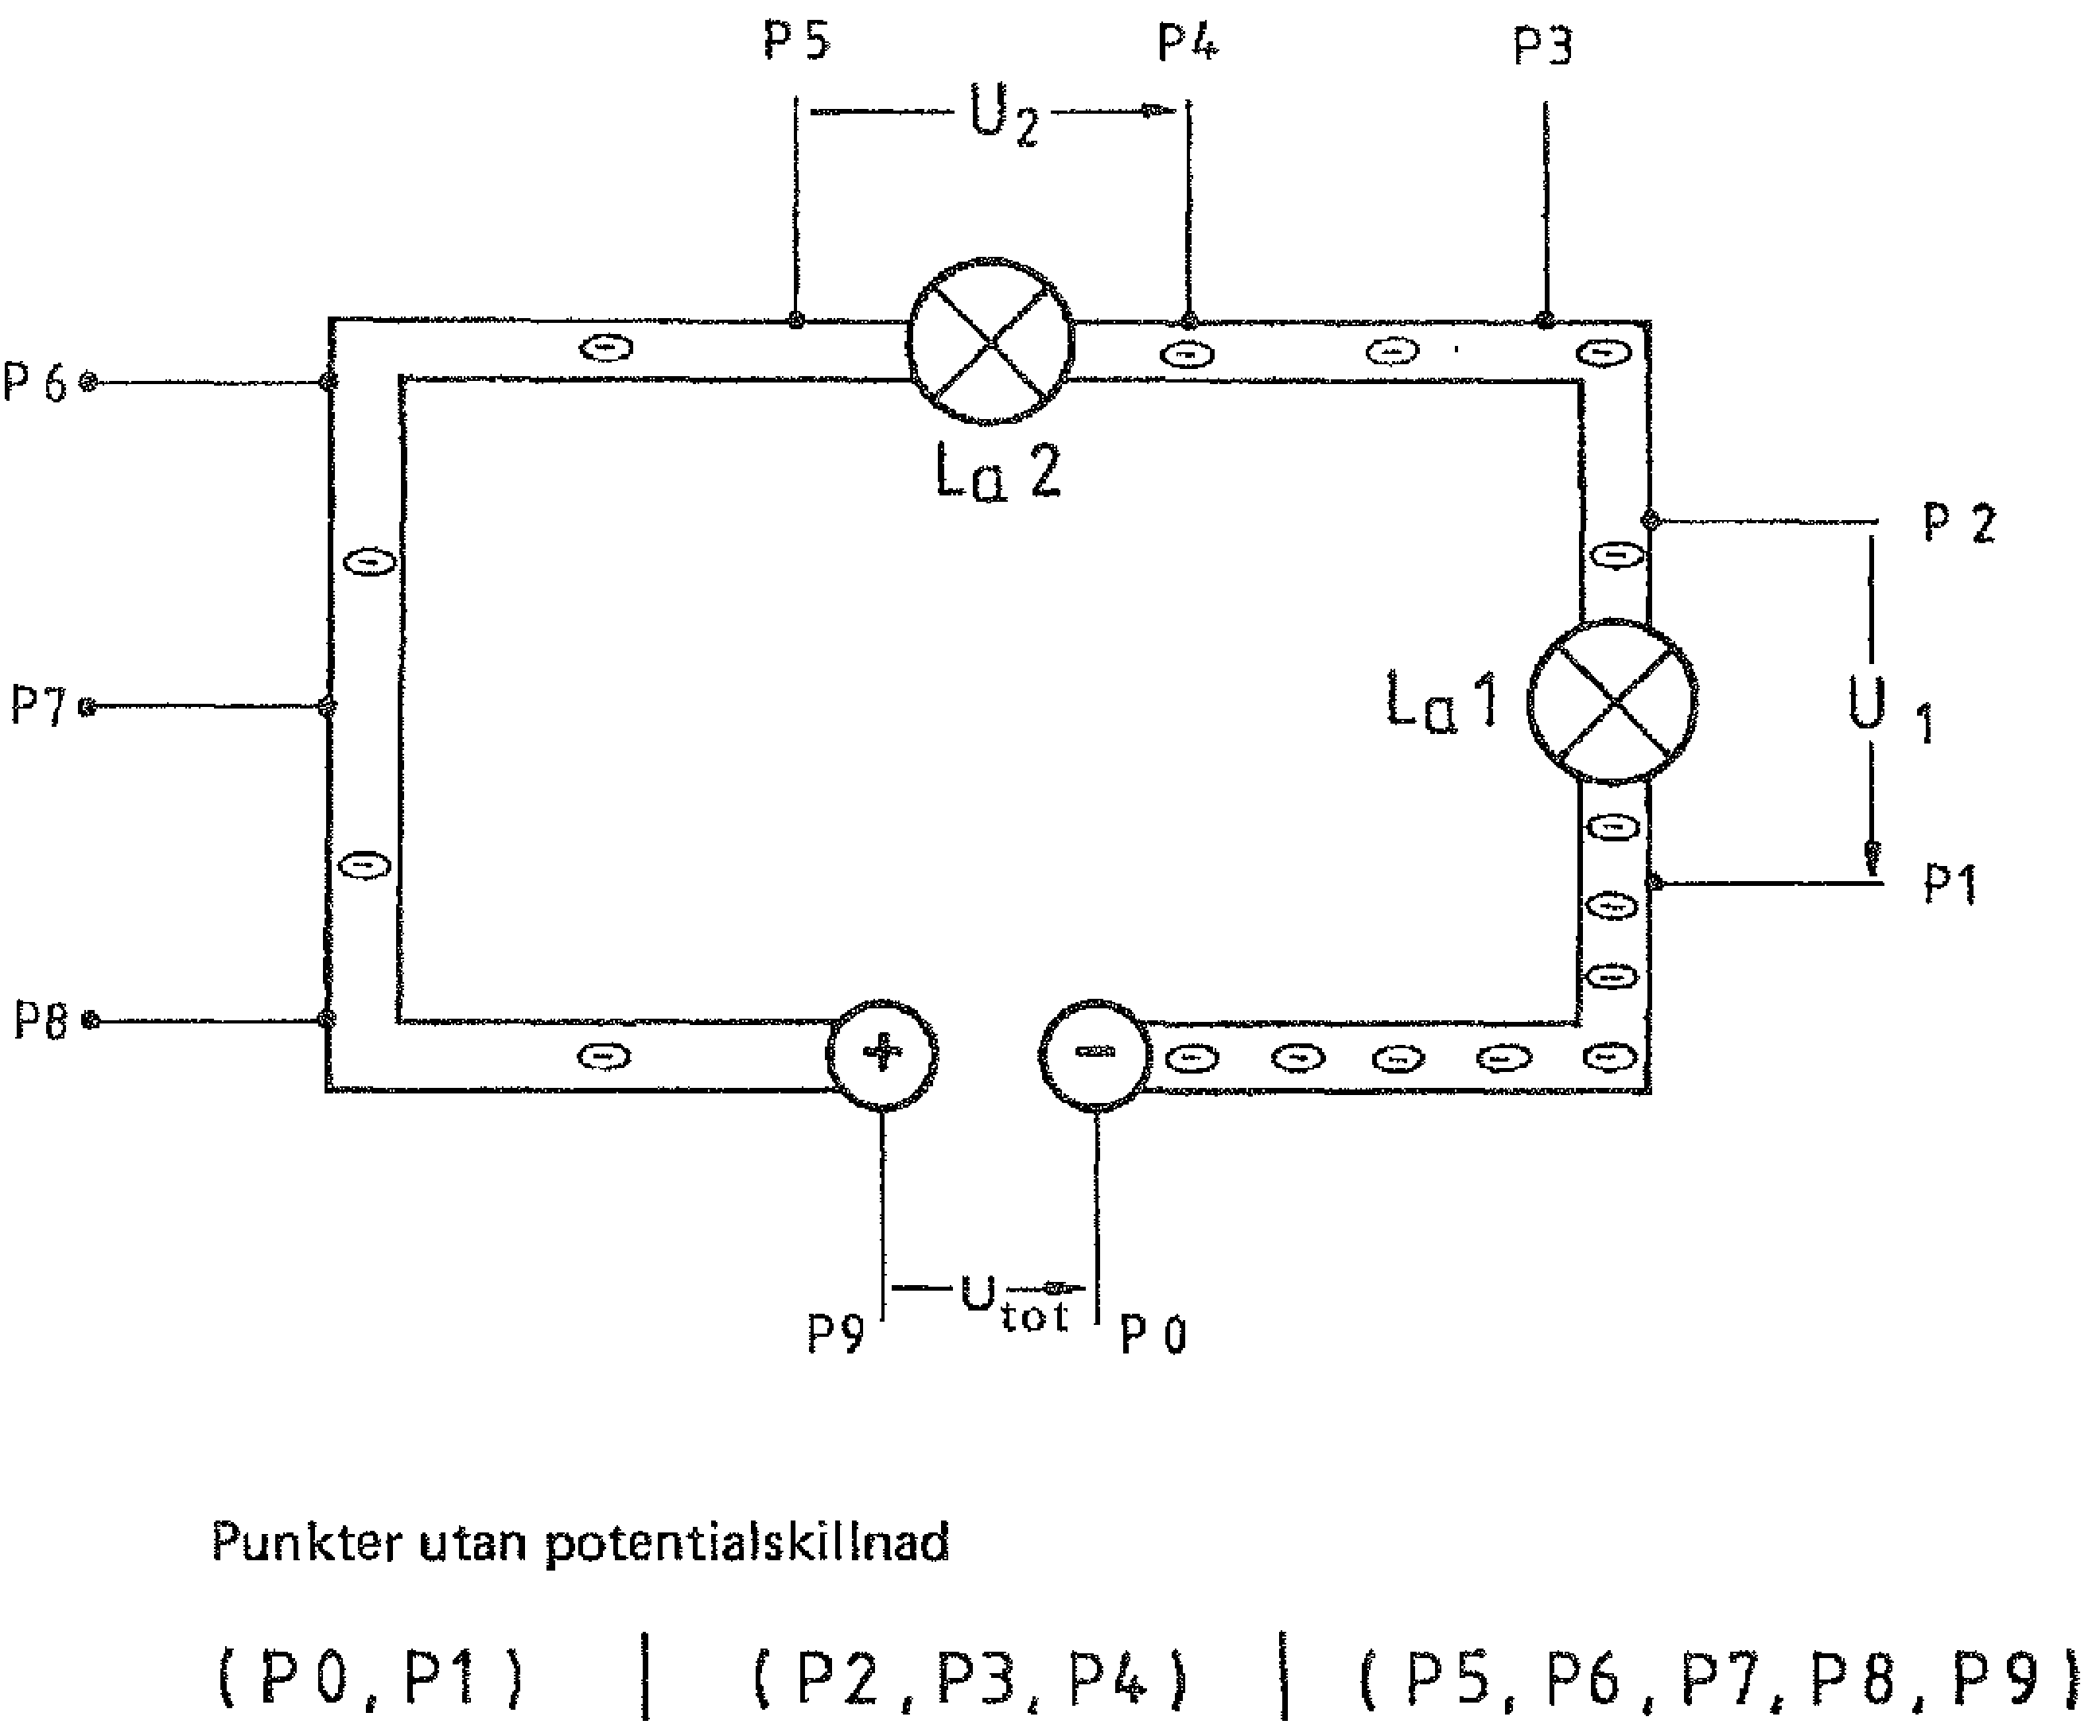
\includegraphics[width=0.6\textwidth]{images/cropped_pdfs/bild_2_1-03.pdf}
\caption{Potential och spänning i en strömkrets}
\label{fig:BildII1-3}
\end{center}
\end{figure*}

Bild \ref{fig:BildII1-3} visar potential och spänning i en strömkrets.

En elektrisk strömkrets består av en eller flera energikällor och
energiförbrukare.
Källor kan vara batterier, nätaggregat etc.
Förbrukare kan vara lampor, ledningar etc.
Varje energiförbrukare har en resistans och de elektriska laddningarna ''köar''
före förbrukaren, strax efter förbrukaren finns ingen kö.
Det uppstår en skillnad i laddningsmängd (en potentialskillnad) mellan varje
punkt i en strömkrets, när det flyter ström.
Man talar om spänningsfall.

\subsection{Strömförlopp}
\textbf{FÖRDJUPNING}
\index{strömförlopp}

Likströms- och växelströmsförloppen kan vara sammansatta av ett huvudförlopp och
underordnade förlopp.

Likström kan ha konstant styrka eller den kan variera enligt något förlopp, men
växlar aldrig riktning.

Växelström kan variera enligt något visst förlopp, t.ex. sinusvåg,
fyrkantsvåg, och växlar ständigt riktning.

\(R_1 \cdot I_1 + R_2 \cdot I_2 + \cdots R_n \cdot I_n = U_1 + U_2 + \cdots U_n\)

\subsection{Resistans -- Enheten Ohm}
\textbf{HAREC a.\ref{HAREC.a.1.1.2}\label{myHAREC.a.1.1.2c}, a.\ref{HAREC.a.1.1.3}\label{myHAREC.a.1.1.3c}}
\index{resistans}
\index{Ohm (\(\Omega\))}
\index{enheter!Ohm (\(\Omega\))}
\index{symbol!\(R\) resistans}

När fria elektroner tvingas fram genom atomstrukturen i en ledare, t.ex.
glödtråden i en lampa, så avgår energi i form av värme.
Detta fenomen kallas för resistans (av latinets resistere som betyder att
motstå).
Resistansen och därmed förlusterna i en strömkrets fördelas i
förhållande till de ingående materialen och deras dimensionering.

Resistans uttrycks i enheten Ohm och betecknas med den grekiska bokstaven
omega (\(\Omega\)).

I formler betecknas resistansen i en elektrisk krets eller en del av den med \(R\).

Resistansen i en resistor är \(1\ \Omega\), när en spänning av \(1\ V\)
driver en ström av \(1\ A\) genom den resistorn.

\subsection{Ohms lag}
\textbf{HAREC a.\ref{HAREC.a.1.1.4}\label{myHAREC.a.1.1.4}}
\index{Ohms lag}
\index{resistor!Ohms lag}

Ohms lag beskriver sambandet mellan grundbegreppen ström \(I\ [ampere]\),
spänning \(U\ [volt]\) och resistans \(R\ [ohm]\).
Sambandet gäller både för likspänning och effektivvärdet för växelspänning och
växelström.

I en ledare med resistansen \(R\) är strömstyrkan \(I\) genom resistansen
proportionell mot den pålagda spänningen \(U\).

\(
\begin{array}{lllll}U=I \cdot R & & I=\dfrac{U}{R} & & R=\dfrac{U}{I}\end{array}
\)

\subsection{Kirchhoffs lagar}
\textbf{HAREC a.\ref{HAREC.a.1.1.5}\label{myHAREC.a.1.1.5}}
\index{Kirchhoffs lagar}
\index{Kirchhoffs strömlag}
\index{Kirchhoffs spänningslag}

Den tyske fysikern G R Kirchhoff (1824--1887) formulerade sina välkända lagar,
först 1845 och sedan 1847.

Kirchhoffs strömlag:

Den algebraiska summan av alla strömmar, som flyter till eller från varje punkt
i en elektrisk krets, är lika med noll.

\(I_1 + I_2 + I_3 + \cdots + I_n = 0\)

Kirchhoffs spänningslag:

I varje sluten strömkrets är den algebraiska summan av alla spänningskällor lika
med det totala spänningsfallet i alla resistorer.

Uttryckt på ett annat sätt är algebraiska summan av spänningarna i en
strömkrets lika med noll.

\subsection{Elektrisk effekt -- Enheten Watt}
\textbf{HAREC a.\ref{HAREC.a.1.1.6}\label{myHAREC.a.1.1.6}, a.\ref{HAREC.a.1.1.7}\label{myHAREC.a.1.1.7}}
\index{elektrisk effekt}
\index{effekt}
\index{Watt (W)}
\index{enheter!Watt (W)}
\index{symbol!\(P\) effekt}

När en ström flyter genom en resistans utvecklas värme.
Värme är en form av effekt, som är högre ju starkare strömmen och högre
spänningen är.

Måttenheten \(voltampere\ [VA]\) för elektrisk effekt härleds ur produkten av
\(volt\ [V]\) och \(ampere\ [A]\).

För effekt som alstras av likström används enheten \(Watt\ [W]\) i stället för
\(voltampere\ [VA]\).
Vid sidan om grundenheten \(1\ W\) används delar och multipler av denna.

\(1\ volt\ [U]\ \cdot\ 1\ ampere\ [I]\ =\ 1\ watt\ [P]\)

Effektformeln \(P = U \cdot I\) kan skrivas om på flera sätt.
Den gäller i första hand för likström men även för växelström om belastningen är
resistiv och ström och spänning inte är fasförskjutna.

\(
\begin{array}{lllll}
U = R \cdot I & & I = \dfrac{U}{R} & & R = \dfrac{U}{I}\\ \\
P = U \cdot I & & P = \dfrac{U \cdot U }{R} & & P = \dfrac{U^2}{R}\\ \\
P = R \cdot I \cdot I & & P = R \cdot I^2 & & U = \sqrt{P \cdot R}
\end{array}
\)

Med hjälp av dessa formler kan effekten beräknas ur resistans- och strömvärdena
respektive ur resistans- och spänningsvärdena.

\subsection{Elektrisk arbete -- Enheten Joule}
\textbf{FÖRDJUPNING}
\index{elektriskt arbete}
\index{Joule (J)}
\index{enheter!Joule (J)}
\index{symbol!\(W\) energi, arbete}

Energi finns i olika former, alltid och överallt.
Energi kan varken skapas eller förstöras, bara omvandlas från en form till en
annan.
Formen kan vara mekanisk, kemisk, elektrisk etc.

Arbete är omvandlingsprocessen från en energiform till en annan.

Arbetsmängden i alla energiformer kan mätas med samma enhet -- \(Joule\ [J]\).

\(1\ Joule\) motsvarar det arbete som utvecklas när ett föremål förflyttas
\(1 meter\) med kraften \(1\ Newton\ [N]\), d. v. s. \(1\ Newtonmeter\ [Nm]\).
Arbetet \([W=Work]\) är mer ju längre tid \([s]\) en viss effekt \([P=Power]\)
utvecklas.

\subsection{Joules lag}
\textbf{HAREC a.\ref{HAREC.a.1.1.8}\label{myHAREC.a.1.1.8}}
\index{Joules lag}

\(Arbete\ =\ Effekt\ \cdot\ tid\)

\([W] = [P] \cdot [s]\)

Eftersom effekten uttrycks som \(P = U \cdot I\) så kan det elektriska arbetet
uttryckas som \(W = U \cdot I \cdot t\), vilket också är Joules lag.

Om grundenheterna för \(volt\ [U]\), \(ampere\ [I]\) och \(sekund\ [s]\) sätts
in i formeln fås en måttenhet, uttryckt som \(voltamperesekunder\ [VAs]\) eller
\(wattsekunder\ [Ws]\) eller \(joule\ [J]\).

Måttenheten för elektriskt arbete är \(1\ Joule\ per\ sekund\), som vanligen
kallas \(1\ wattsekund\ [1\ Ws]\).
Vid sidan av grundenheten används multipler av denna.
Exempel:
\(
\begin{array}{llll}
1\ kilowattsekund & = 1\ kWs & = 1\ 000\ Ws & = 1,0 \cdot 10^3\ Ws\\
1\ wattimme & = 1\ Wh & = 3\ 600\ Ws & = 3,6 \cdot 10^3\ Ws \\
1\ kilowattimme & = 1\ kWh & = 1 000\ Wh & = 3,6 \cdot 10^6\ Ws
\end{array}
\)

\subsection{Formelsnurran}
\index{formelsnurran}
\textbf{FÖRDJUPNING}

\begin{figure*}[ht]
\begin{center}
  %%\begin{wrapfigure}{R}{0.3\textwidth}
  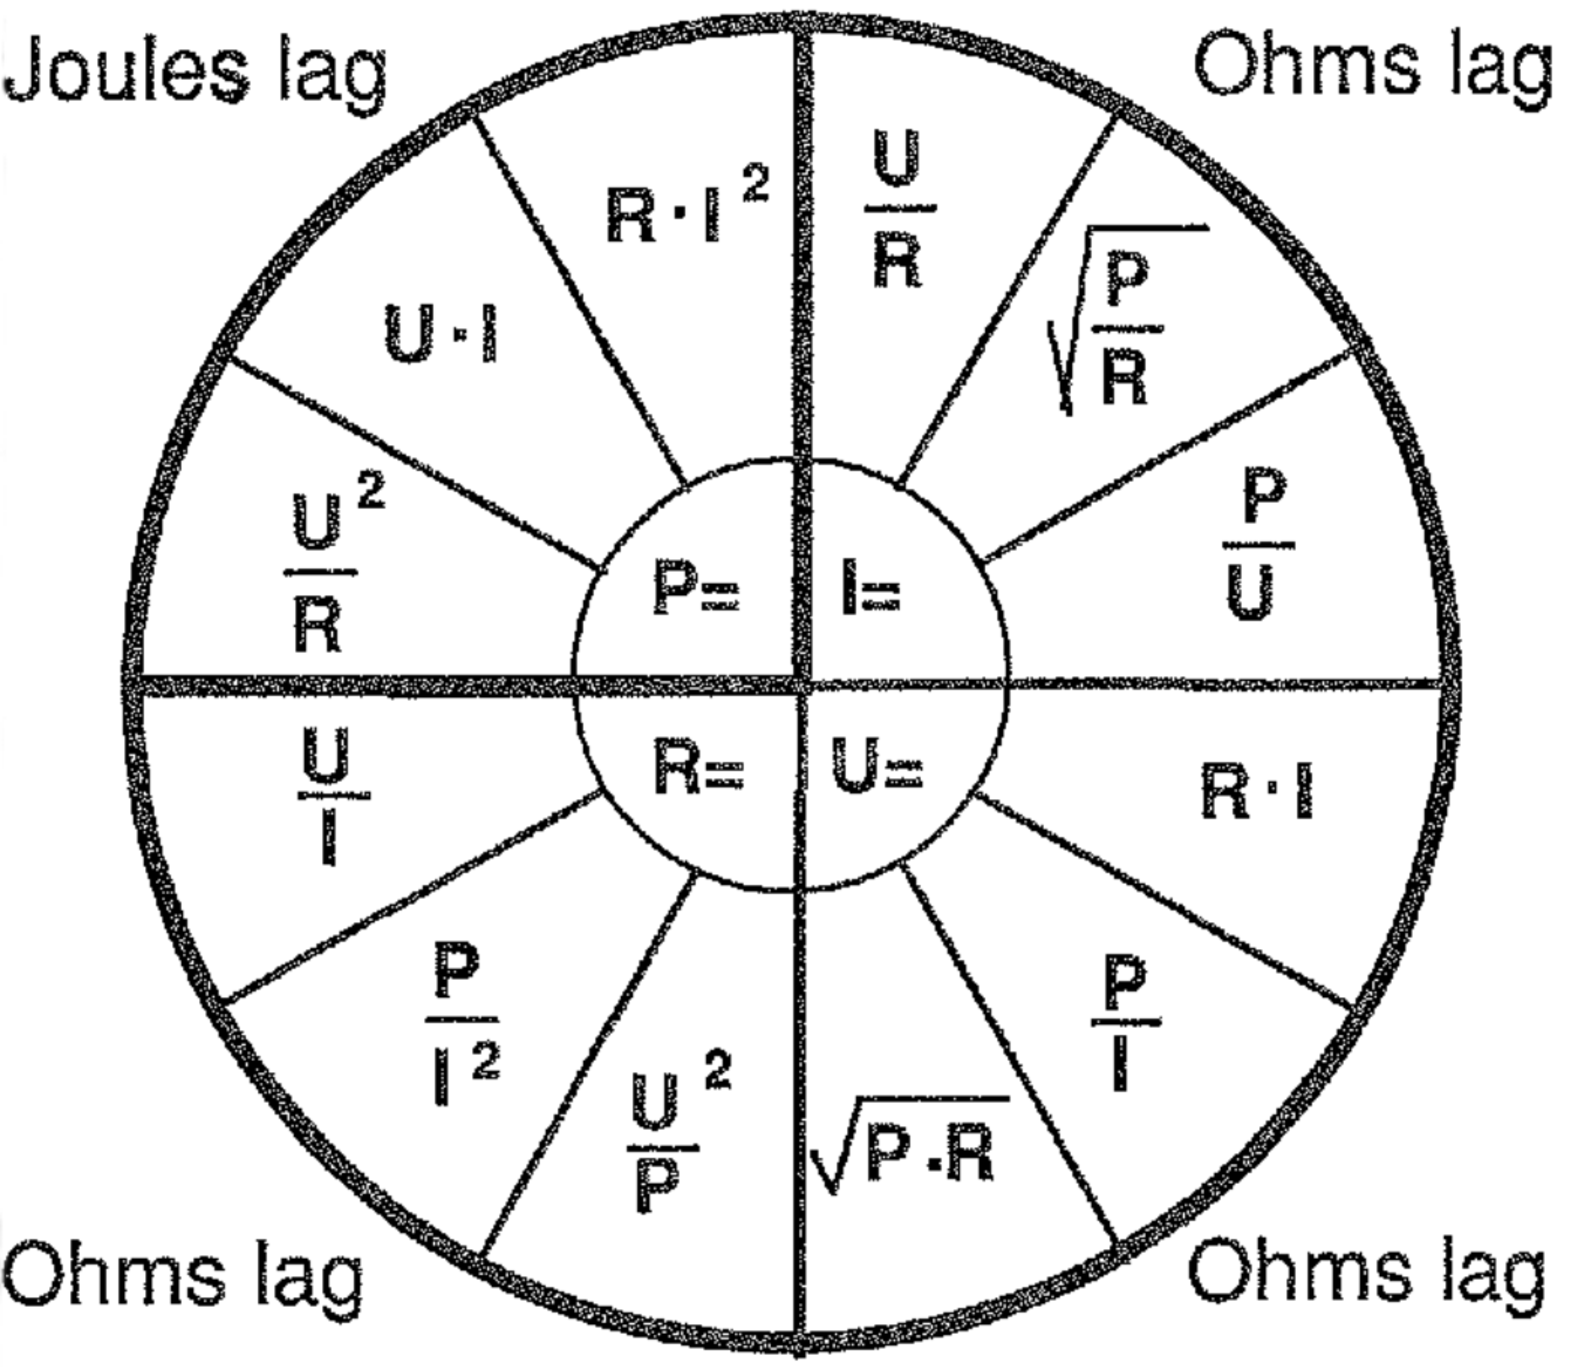
\includegraphics[width=0.5\textwidth]{images/cropped_pdfs/bild_2_1-04.pdf}
  \caption{''Formelsnurra'' för Ohms och Joules lagar}
  \label{fig:BildII1-4}
  %  \vspace{-100pt}
  %%\end{wrapfigure}
\end{center}
\end{figure*}

Så här finner man rätt formel i ''snurran'' (bild \ref{fig:BildII1-4}):
Välj ett segment med önskad storhet \(I\), \(U\), \(R\) eller \(P\) som det
första ledet i formeln.
Inom valt segment finns tre alternativ för det andra ledet i formeln.
Välj det alternativ som innehåller två kända storheter.

Bild \ref{fig:BildII1-4} visar ''Formelsnurra'' för Ohms och Joules lagar.

Exempel:

\subsubsection{Ohms lag}

\(R\) söks, \(U\) och \(I\) är kända;
Om \(U = 230\ V\) och \(I = 2\ A\), så blir

\(R=\dfrac{U}{I}=\dfrac{230}{2}=115\ \Omega\)

\subsubsection{Joules lag}

\(P\) söks, \(U\) och \(I\) är kända;

Om \(U = 230\ V\) och \(I = 2\ A\), så blir

\(P = U \cdot I = 230 \cdot 2 = 460\ W\)

\subsection{Amperetimmar (Ah) och batterikapacitet}
\textbf{HAREC a.\ref{HAREC.a.1.1.9}\label{myHAREC.a.1.1.9}}
\index{Amperetimmar (Ah)}
\index{batterikapacitet}

Det finns flera sätt att lagra energi.
Ett sätt är att göra det i kemisk form i speciella celler, där man kan ta ut
energin i elektrisk form.

Det finns celler som kan laddas upp och laddas ur upprepade gånger, s.k.
ackumulatorer.
Det finns också sådana celler som endast kan användas en gång och som inte
kan laddas upp igen, s.k. primärceller.

Energi i form av en elektrisk laddning kan även lagras i en kondensator.
Energin kan då lagras och tas ut utan omvandling.

Kapaciteten i en elektrisk cell uttrycks som produkten av den ström \([A]\) som
cellen avger och under den tid \([s, h]\) detta kan ske.
Uttryckt med tidsenheten timmar blir då kapaciteten \(Ah\).

Den kapacitet som anges i en cells produktdata är den nominella.
Denna kapacitet gäller endast under vissa normerade förhållanden såsom
celltemperatur, strömstyrka och urladdningstid.

Den praktiska kapaciteten i en cell begränsas av användningen.
En elektrisk cell avger sålunda regelmässigt mindre energimängd, desto högre
urladdningsströmmen är.
Kapaciteten i en elektrisk cell skiljer sig i det avseendet från den i
t.ex. en oljetank, där man kan ta ut lika mycket energimängd som man häller i
och oberoende av hur fort man gör det.

Elektriska celler kan samlas till s.k. batterier, varvid cellerna oftast
seriekopplas.
Batteriets polspänning är då summan av cellernas polspänningar.

Hur stort arbete ett batteri avger, beror då såväl på hela batteriets
polspänning som på de enskilda cellernas kapacitet.
Exempel:
Ett batteri med polspänningen \(12\ V\) och cellkapaciteten \(100\ Ah\) kan
nominellt avge
\(P = U \cdot I = 12 \cdot 100 = 1200\ VAh = 1,2\ kWh\).

Hur länge batteriet ''räcker'' per laddning beror som sagt bl.a. på vilken
strömstyrka man tar ut.
Tar man ut \(1\ A\) ur \(100\ Ah\)-cellen här ovan, så blir urladdningstiden
nominellt \(t = 100\ Ah/1\ A = 100\ h\).
